\documentclass[12pt]{report}
\usepackage[utf8]{inputenc}
\usepackage[T1]{fontenc}
\usepackage[francais]{babel}
\usepackage{titlesec}
\usepackage{amsmath}
\usepackage{amssymb}
\usepackage{layout}
\usepackage{graphicx}
\usepackage[top=2cm, bottom=2cm, left= 2.5cm, right=2.5cm]{geometry}

\title{Projet Advance Wars}
\date{\today}
\author{Pierre MARIET - Joanna XANH\\
3\up{ème} année, Option Informatique et Systèmes}
\begin{document}

\begin{figure}

\includegraphics[width=60mm, height=65mm]{logoENSEA.png}
\end{figure}

\maketitle
\thispagestyle{empty}
\newpage

\tableofcontents
\newpage

\chapter{Présentation générale}
    \section{Archétype}
    \paragraph{}Le projet est de recréer le jeu Advance Wars\textsc{\texttrademark} développé par Intelligent Systems\up{\textregistered} pour la Game Boy Advance\textsc{\texttrademark} de Nintendo\up{\textregistered}.\newline
    Le jeu est en tour par tour, sur une carte découpée en cases. Les cartes pourront être crées à partir d'un fichier texte.
    \section{Règles du jeu}
    \subsection{Description des unités}
    \paragraph{}Sur une carte composée de différents terrains et séparée en cases s'affrontent 2 armées. Les terrains augmentent ou non la défense de l'unité qui se trouve dessus. Ces armées sont composées de différentes unités qui ont chacune des spécificités qui varient :
    \begin{itemize}
        \item Les unités aériennes peuvent se déplacer n'importe où sur la carte. Les unités de transport aérien ont une capacité de 1 et ne peuvent débarquer en mer ou en montagne.
        \item Les unités navales ne peuvent se déplacer qu'en mer, pas dans les rivières. Les unités de transport naval peuvent débarquer uniquement sur une plage ou dans un port.
        \item Les unités d'infanterie et bazookas peuvent se déplacer sur tous les sols et traverser les rivières.
        \item Les unités terrestres motorisées ne peuvent franchir les montagnes.
    \end{itemize}
    \subsection{Les généraux et leurs pouvoirs}
    \paragraph{}Chaque armée est dirigée par un général possédant un pouvoir qui donne un avantage à son armée ou un inconvénient à l'ennemi. Ce pouvoir dure un tour (sauf dans pour le Blizzard) et se recharge sur plusieurs tours. Le général donne en plus un avantage moindre, ou non, mais en rapport avec son pouvoir et qui dure toute la partie.
    
    
        \paragraph{Réparation}Redonne 2 points de vie à toutes les unités alliées. Aucune autre spécificité en dehors du pouvoir.
        Les statistiques de ce général représentent les statistiques moyennes.
        
        \paragraph{Blizzard}Provoque une tempête de neige qui dure deux tours et qui diminue l'amplitude de déplacement des unités adverses.
        Aucune autre spécificité en dehors du pouvoir.
        
        \paragraph{Marche forcée}L'infanterie peut se déplacer d'une case en plus et les bazookas ont une force de frappe augmentée de 50\%.
        Par défaut, l'infanterie et les bazookas ont un bonus de force de frappe de 20\% et de 10\% de défense contre les unités d'infanterie adverse. Une unité qui capture un bâtiment a vitesse de capture de 150\% de ses points de vie.
        La puissance de frappe des autres unités de tir direct est en revanche moins élevée que la moyenne. Les unités de transports peuvent se déplacer d'une case en plus par rapport à la moyenne.
        
        \paragraph{Puissance Max}Les chars d'assaut voient leur puissance de frappe augmenter de 140\%, leur défense augmente de 1 point et leur amplitude de déplacement augmente de 1 case.
        Par défaut, les chars d'assaut ont une puissance de frappe 150\% plus élevée que la moyenne.
        
        \paragraph{Embuscade}Les unités de tir indirect voient leur portée augmenter de 1 et leur force de frappe augmenter de 150\%.
        Par défaut, la portée des unités de tir indirect est augmentée de 1 case. Les unités de tir direct ont une force de frappe diminuée de 20\%.
        
        \paragraph{Frappe éclair}Les unités aériennes peuvent se déplacer une nouvelle fois pendant le tour.
        Par défaut, la force de frappe des unités aériennes est 15\% plus élevée que la moyenne Les forces navales ont une force de frappe réduite de 20\% par rapport à la moyenne.
        
        \begin{figure}[h]
    \begin{center}
    
\includegraphics{advance_wars_sprites_andy.png}
    
\includegraphics{advance_wars_sprites_olaf.png}
    
\includegraphics{advance_wars_sprites_sami.png}
    
\includegraphics{advance_wars_sprites_max.png}
    
\includegraphics{advance_wars_sprites_eagle.png}
    
\includegraphics{advance_wars_sprites_gritt.png}
    \end{center}
    \caption{Sprites des généraux}
    \end{figure}
    
    \section{Ressources}
    \paragraph{}Les ressources graphiques utilisées sont celles du jeu d'origine. Néanmoins, en considérant le temps de développement des autres paramètres du jeu, seuls la carte, les unités sur celle ci ainsi que les animations de capture seront affichées.
    
    \begin{figure}[h]
    \begin{center}
    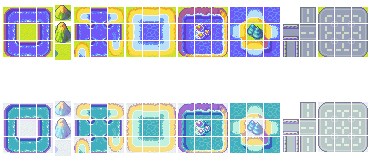
\includegraphics{advance_wars_sprites_map_tiles.png}
    \end{center}
    \caption{Sprites pour les tuiles de la carte}
    \end{figure}
    
    \begin{figure}[h]
    \begin{center}
    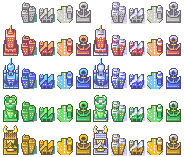
\includegraphics{advance_wars_sprites_cities.png}
    \end{center}
    \caption{Sprites des différents batiments de la carte}
    \end{figure}
    
    \begin{figure}[h]
    \begin{center}
    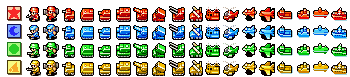
\includegraphics{advance_wars_sprites_units.png}
    
\includegraphics[scale=1.8]{advance_wars_sprites_units_info.png}
    \end{center}
    \caption{Sprites des unités ainsi que les informations de statut}
    \end{figure}
    
    \begin{figure}[h]
    \begin{center}
    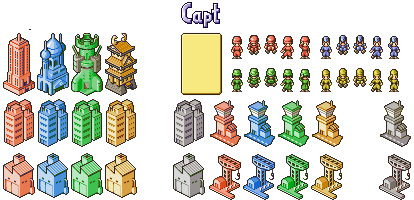
\includegraphics{advance_wars_sprites_capture.png}
    \end{center}
    \caption{Animations de capture}
    \end{figure}
    
    \begin{figure}[h]
    \begin{center}
    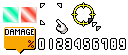
\includegraphics{advance_wars_sprites_damages.png}
    \end{center}
    \caption{Sprites des fenêtres d'attaque}
    \end{figure}
\end{document}
